%!TEX root = thesis.tex

\newpage

\chapter{Обзор реализованного программного обеспечения}

Для решения поставленной задачи, в рамках данной работы, было реализовано клиент-серверное приложение, позволяющее решать класс аналогичных по структуре задач. Для этого написаны несколько модулей, включающих в себя функционал, необходимый для решения конкретной подзадачи. Для удобства работы, каждый модуль имеет отдельные страницы, отвечающие за конкретные инструменты. Таким образом весь процесс работы в приложении разбивается на несколько этапов, на каждом из которых решается конкретная подзадача. В данной работе можно выделить три этапа: первичный анализ данных, анализ остатков и вариограммный анализ. Дальше в данной главе будет рассмотрены подробнее каждый из аспектов реализации.

Следует отметить, что каждая страница приложения имеет единый дизайн: экран можно условно поделить на панель выбора этапа анализа сверху и область исследования снизу. В свою очередь область исследования можно разделить также на две части: контрольная панель параметров и инструментов слева, и результаты вычислений и анализа справа.

\section{Модуль первичного анализа} % (fold)
\label{sec:mod_basis}

Данный модуль включает в себя возможности по просмотру и анализу непосредственно данных: графически и с помощью таблицы, позволяющей сортировать и производить поиск по определённому признаку. Непосредственно на рисунке \ref{img:mod_basis} отображена вкладка первичного анализа.
\begin{figure}[ht]
\center{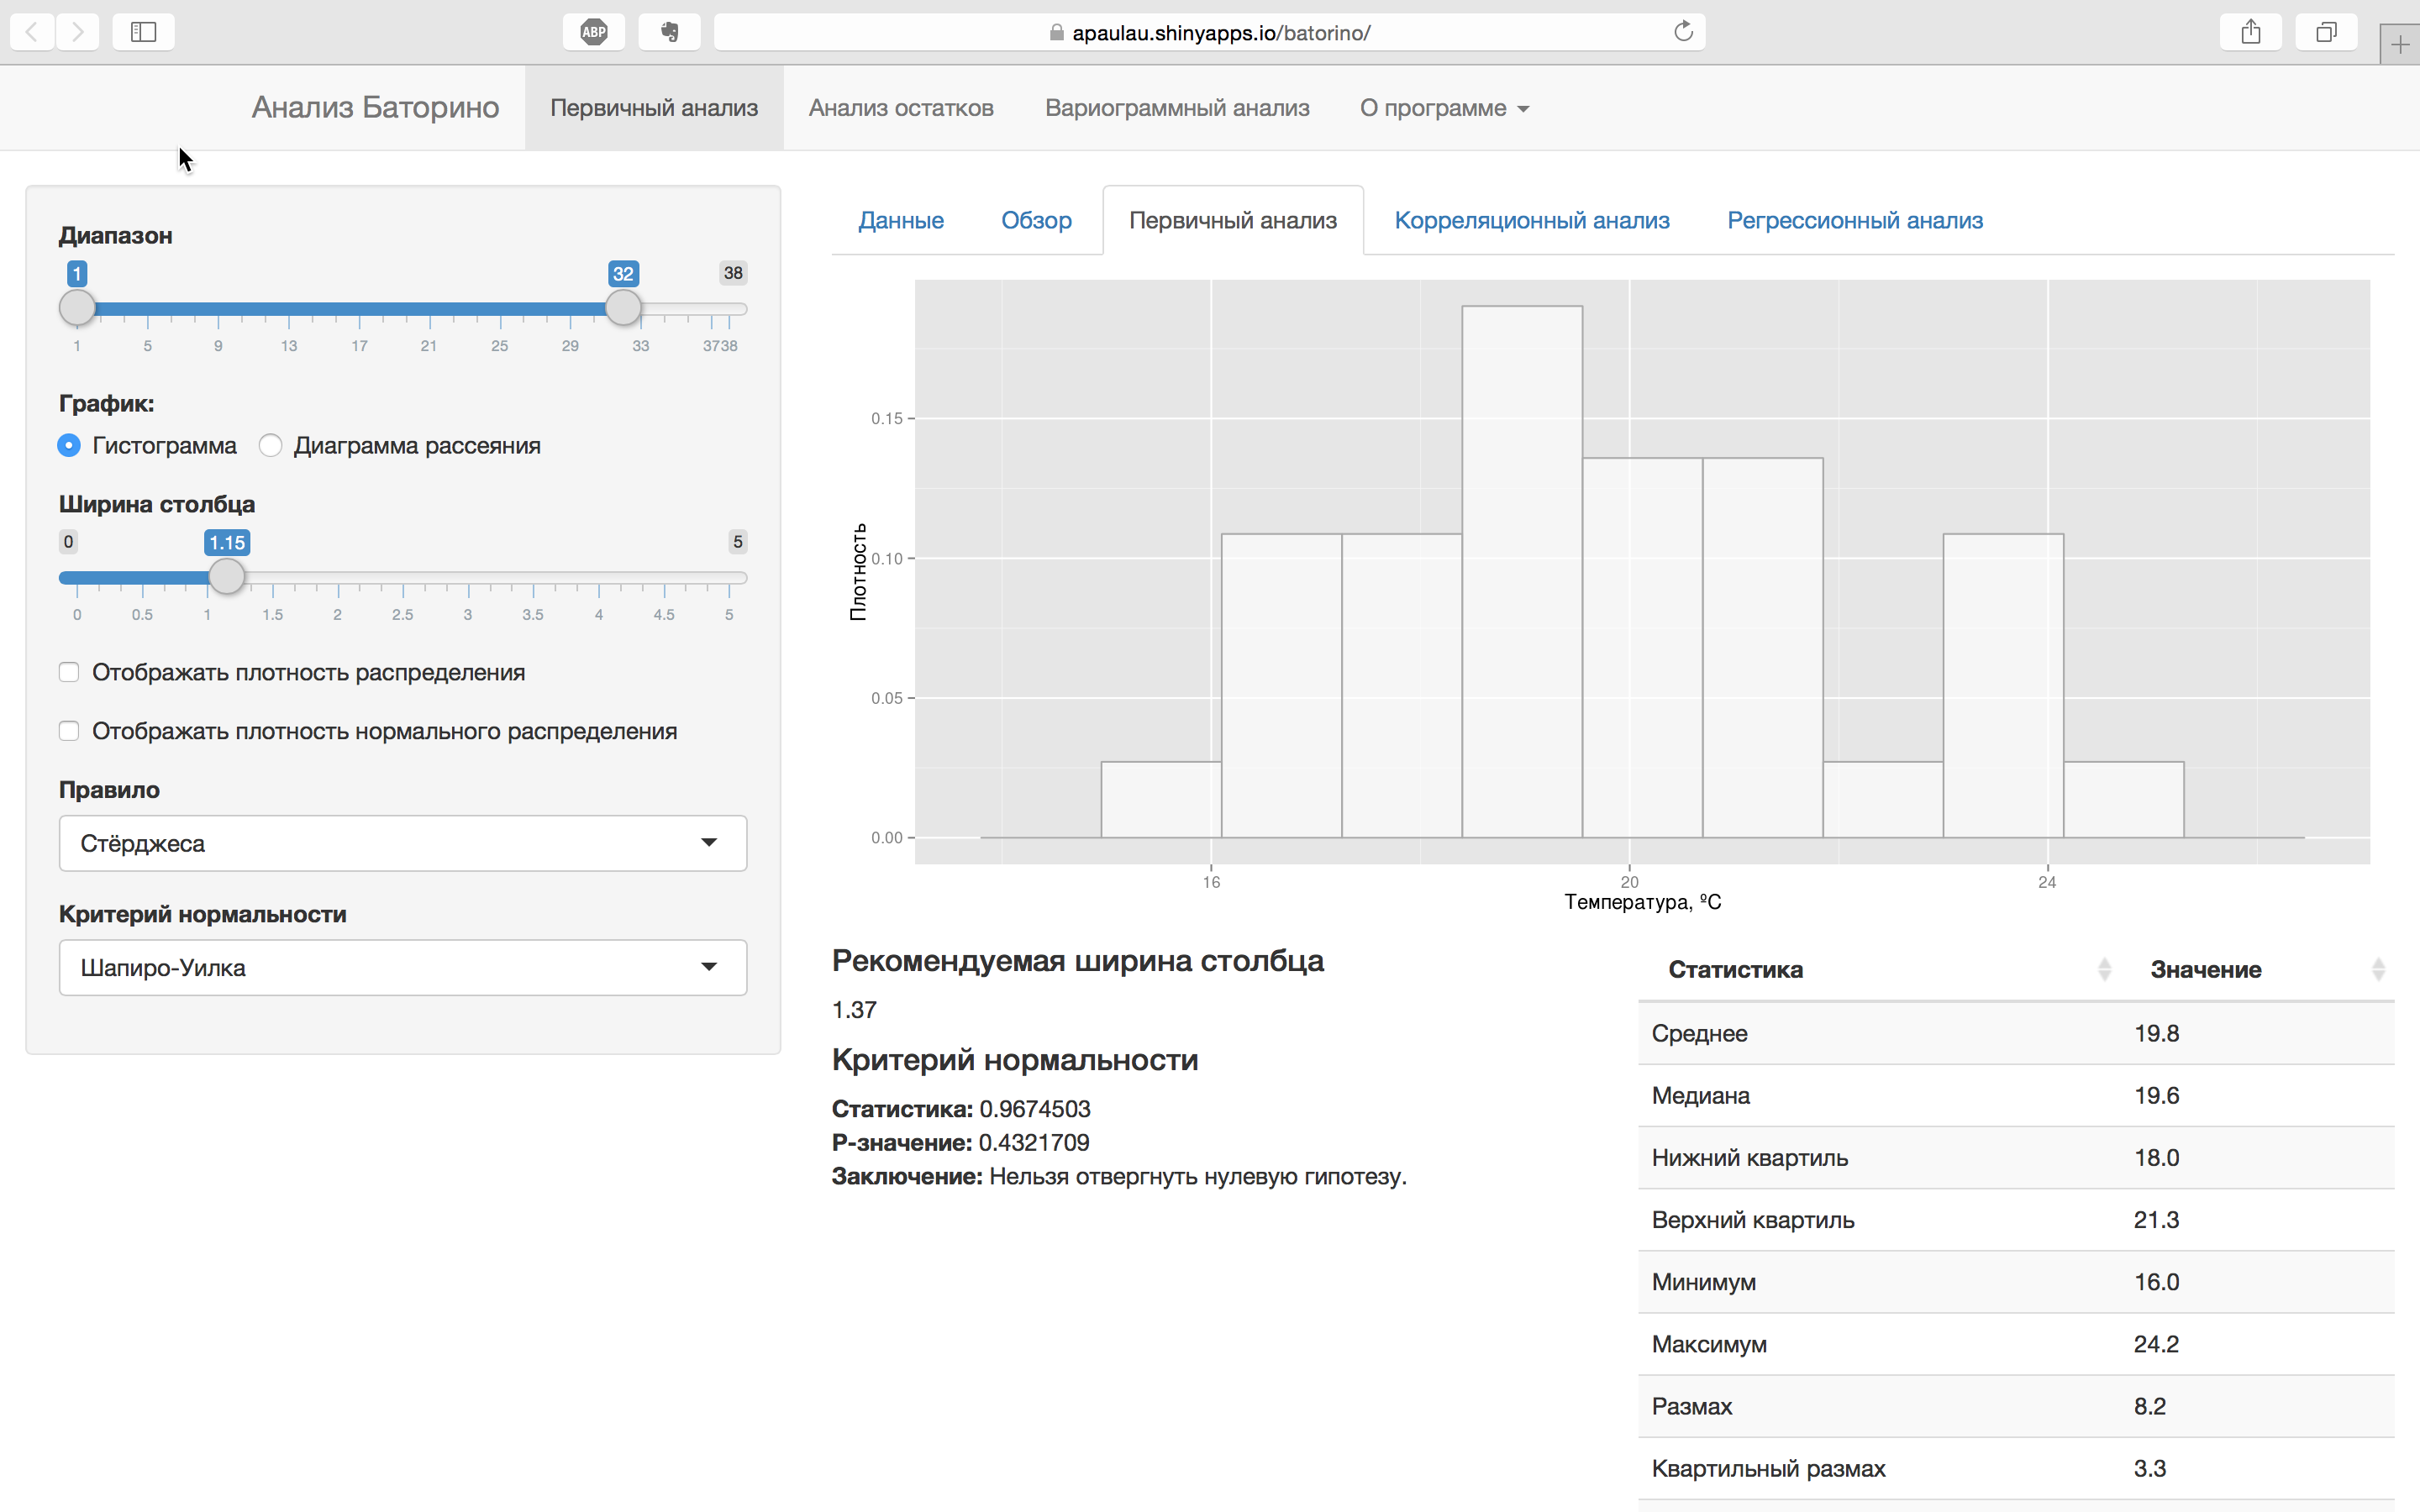
\includegraphics[width=1\linewidth]{../figures/static/1_basis.png}}
\caption{Первичный анализ и описательные статистики}
\label{img:mod_basis}
\end{figure}
В которой представлены возможности по определению закона распределения исследуемых данных с помощью как проверки различными тестами, так и визуально, на гистограмме и графике квантилей. Контрольная панель позволяет изменять отображаемый в данный момент график, а также позволяет выбрать критерий нормальности. В случае выбора для отображения гистограммы, появляются управляющие элементы, позволяющие выбрать ширину столбца на гистограмме и правило по её вычислению (например, правило Стерджеса), отобразить плотность выборочного распределения и кривую нормального. Также на данной странице вычисляются описательные статистики, отображённые в виде таблицы.

Следующей вкладкой в данном модуле является корреляционный анализ. Данная страница позволяет оценить зависимость исследуемых данных с помощью диаграммы рассеяния, вычисляет коэффициент корреляции и с помощью критерия Стьюдента проверяет значимость вычисленного коэффициента, а также вычисляет для него доверительный интервал. Среди прочего, данная страница позволяет оценить наличие выбросов с помощью критерия Граббса.

Вкладка регрессионного анализа (рисунок \ref{img:mod_regr}) позволяет получить регрессионную модель по исследуемым данным. График временного ряда содержит также линию регрессии.
\begin{figure}[ht]
\center{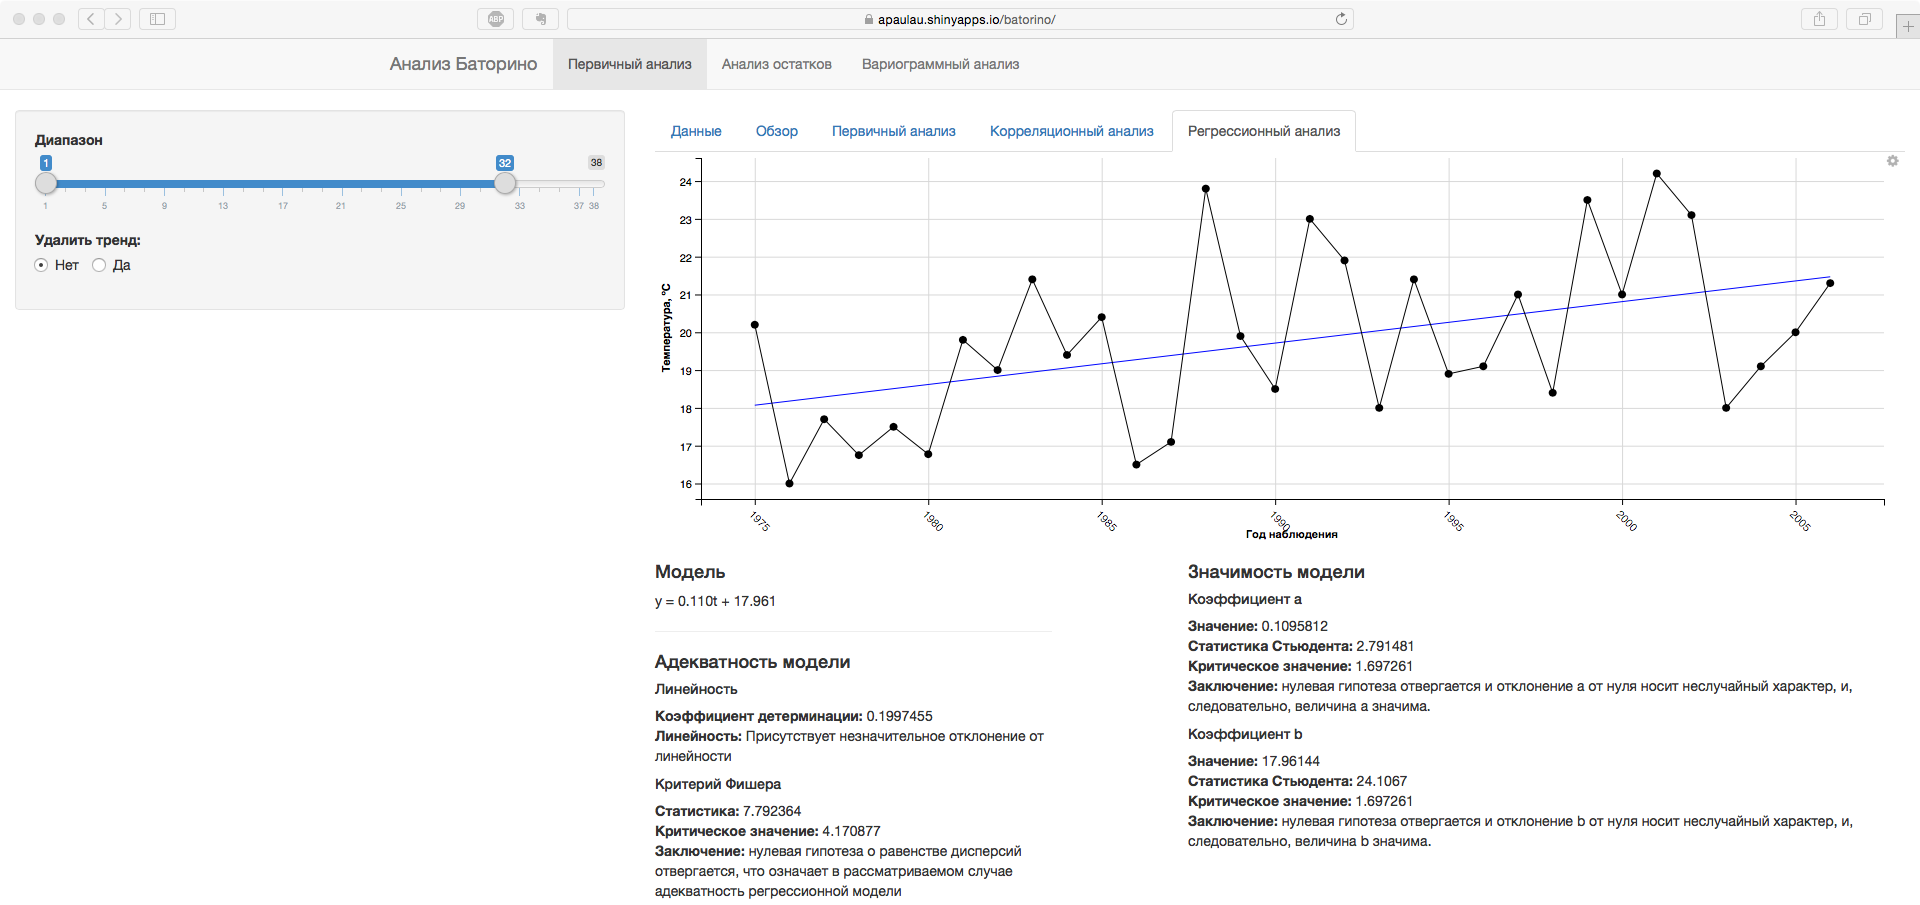
\includegraphics[width=1\linewidth]{../figures/static/2_regr.png}}
\caption{Регрессионный анализ}
\label{img:mod_regr}
\end{figure}
Представленная страница демонстрирует возможности по анализу вычисленной модели: определение значимости вычисленных коэффициентов, адекватность модели с помощью критерия Фишера и проверки линейности.

Инструменты, рассмотренные в рамках данного модуля, позволяют быстро получить информацию по исследуемым данным. А также сделать первые выводы и наметить шаги по дальнейшему исследованию. Заметим, что на каждом из этапов анализа и использования каждого из инструментов реализована возможность изменять объёмы выборки. Как снизу, так и сверху. Другими словами можно отбросить первые или последние наблюдения. Это позволяет быстро оценить, насколько влияют данные на результат в конкретном случае.

% section mod_basis (end)

\section{Модуль анализа остатков} % (fold)
\label{sec:mod_residuals}

Данный модуль является логическим продолжением рассмотренного ранее. После регрессионного анализа и удаления из исходного временного ряда тренда, основанного на регрессионном уравнении, получаем ряд остатков. Для его анализа реализованы возможности, которые включают в себя некоторые возможности предыдущего. Исключение составляют инструменты регрессионного и корреляционного анализов. Поскольку исследуемый на данном этапе временной ряд не имеет явных составляющих.

Таким образом данный модуль позволяет проверить остатки на нормальность как с помощью графиков квантилей и гистограммы, так и различными критериями: Шапиро-Уилка, $ \chi^2 $-Пирсона, Колмогорова-Смирнова. В дополнение к этому имеется возможность проанализировать описательные статистики, а также исследовать автокорреляционную функцию. Страница с таким инструментом представлена на рисунке \ref{img:mod_acf}.
\begin{figure}[ht]
\center{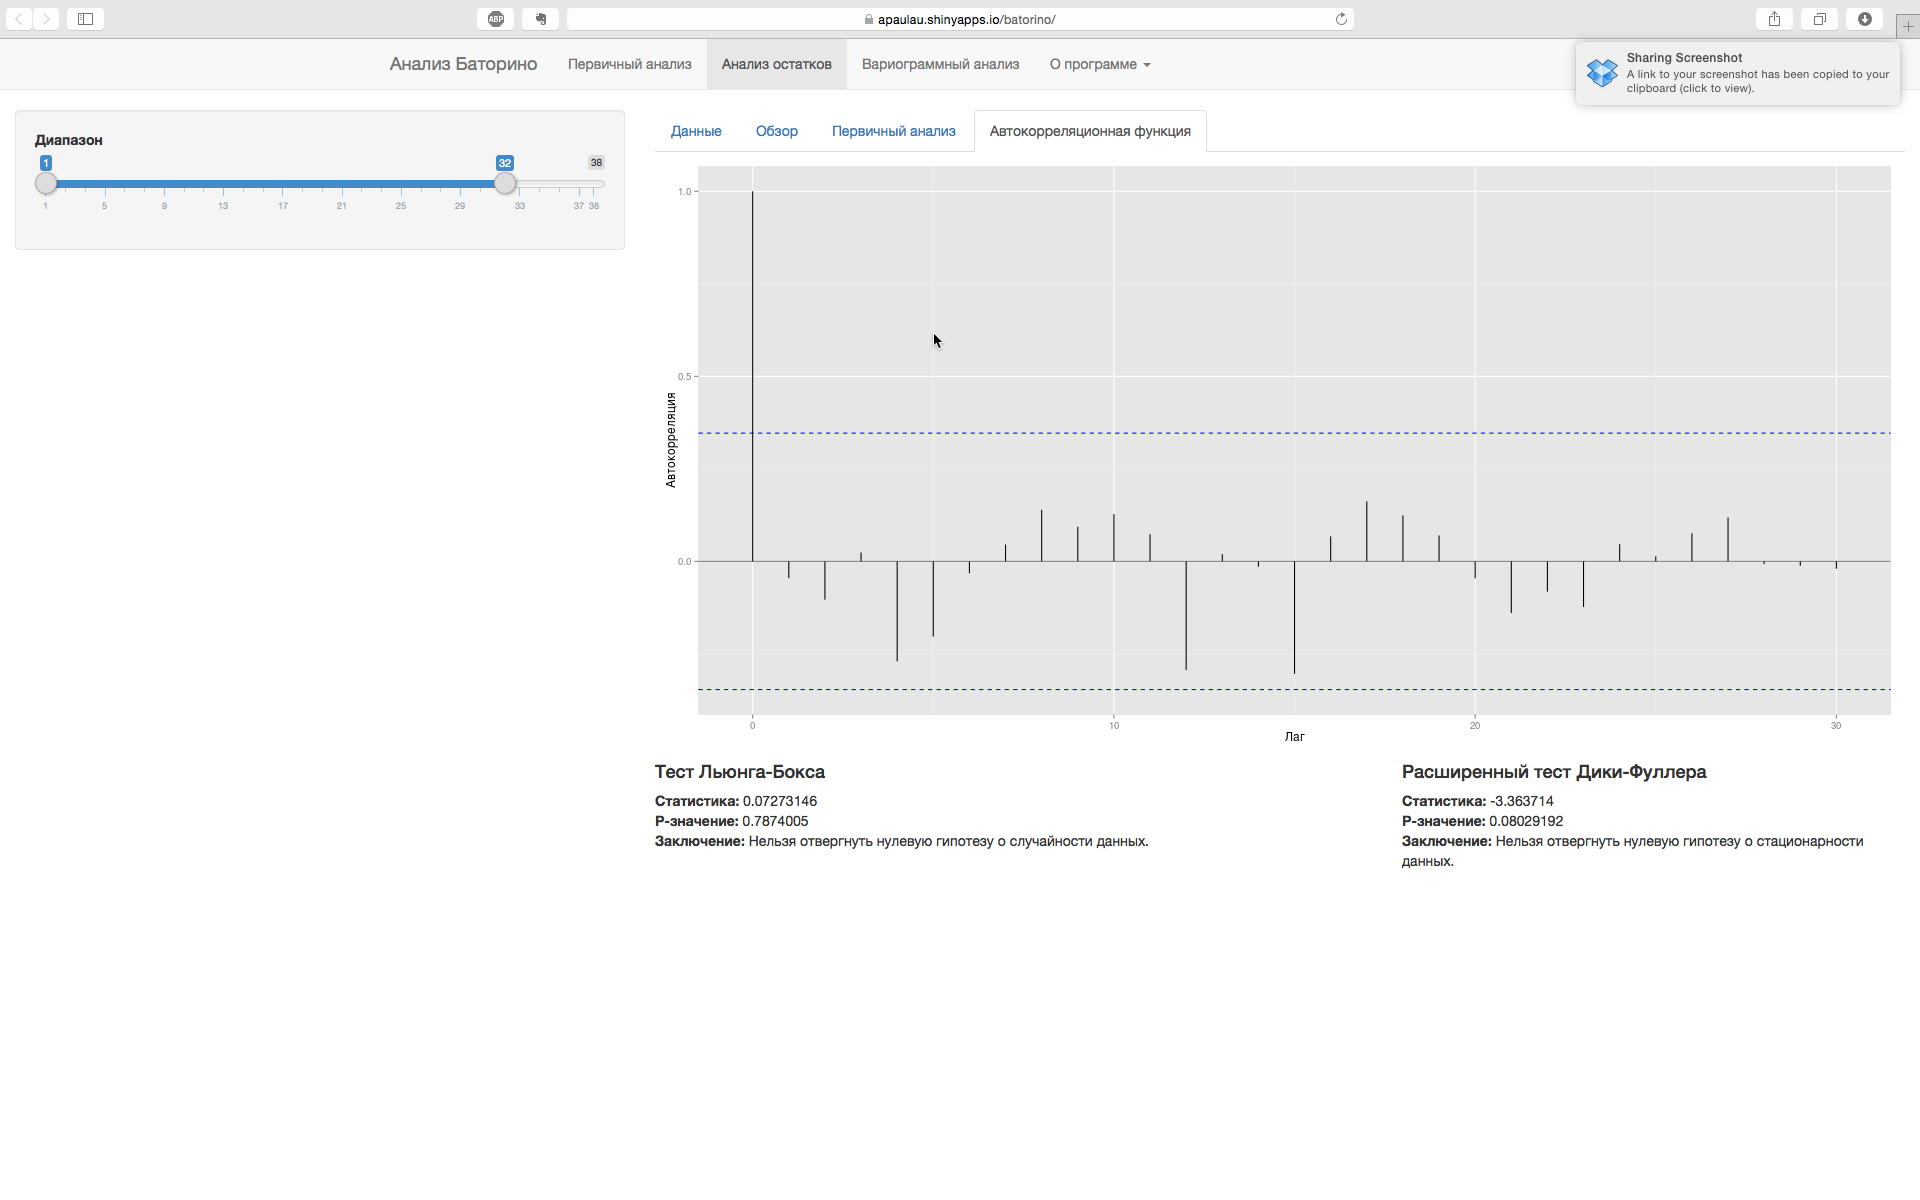
\includegraphics[width=1\linewidth]{../figures/static/3_acf.png}}
\caption{Анализ автокорреляционной функции}
\label{img:mod_acf}
\end{figure}
На рисунке продемонстрирован график автокорреляционной функции, позволяющий визуально определить наличие автокорреляций в исследуемых данных. Также проверить наличие значимых автокорреляций позволяет проверка реализованного теста Льюнга-Бокса. В свою очередь, расширенный тест Дики-Фуллера, также представленный на рассматриваемой странице, проверяет наличие стационарности в исследуемом случайном процессе.

В зависимости от результатов, полученных на рассмотренном этапе, можно либо закончить исследование, либо продолжить в модуле вариограммного анализа. Закончить исследование стоит в том случае, если ряд остатков полностью характеризуется как случайный шум, либо в случае, когда не выполняются условия для проведения следующего этапа.

% section mod_residuals (end)

\section{Модуль вариограммного анализа} % (fold)
\label{sec:mod_variogram}

В данном модуле используются современные геостатистические методы и инструменты, которые, в рамках \textbf{R}, реализованы пакетом \textit{gstat}. В этом пакете представлены функции для вычисления вариограмм, подбору моделей и параметров, интерполирования методами кригинга и методы валидации конечных результатов. Интерполирование методами кригинга подразумевает наличие подобранной модели вариограммы, поэтому в рассматриваемом модуле акцент сделан именно на подборе и анализе различных моделей вариограмм.

Начальный шаг состоит в подборе модели и её параметров к экспериментальной вариограмме. Для построения экспериментальной вариограммы присутствует возможность использовать две разновидности оценок вариограммы: рассмотренная в главе 2 оценка Матерона и робастная оценка Кресси-Хокинса. Для подбора модели вариограммы, в общем случае, существует два подхода: подбор визуально вручную, силами исследователя, и автоматическими методами. В данном модуле в полной мере реализованы оба подхода. В первом случае, изменение любого из параметров модели позволяет незамедлительно оценить эффект как на графике непосредственно вариограммы, так и по конечному прогнозу кригингом.

На рисунке \ref{img:mod_variogram} скриншот начального этапа вариограммного анализа. Инструменты данной страницы позволяют выбрать модель из следующих: Линейная, Сферическая, Экспоненциальная, Гауссовская, Круговая, Бесселя, Пентасферическая, Волновая, Логарифмическая. А также задать к выбранной модели параметры.
\begin{figure}[ht]
\center{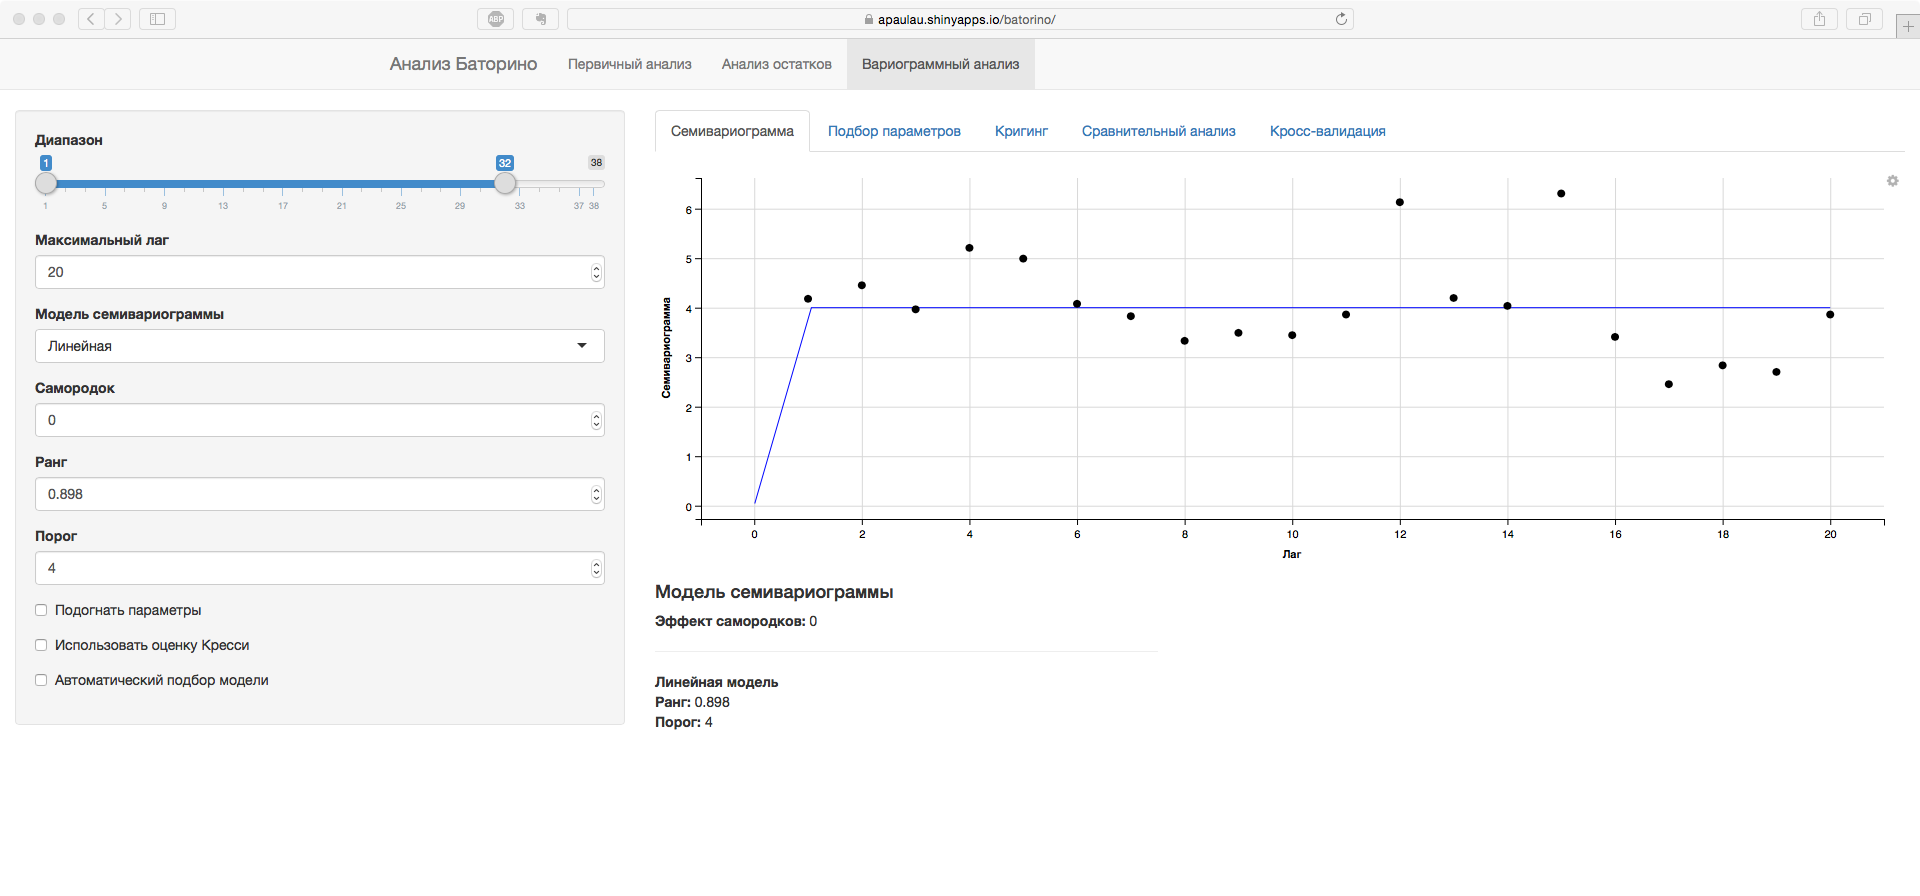
\includegraphics[width=1\linewidth]{../figures/static/4_variogram.png}}
\caption{Возможности по подбору модели вариограммы}
\label{img:mod_variogram}
\end{figure}
Заданные параметры считаются начальными, если выбрать опцию подгона методом наименьших квадратов. На этом шаге также можно воспользоваться реализованным в рамках данной работы алгоритмом автоматического подбора модели. Данная функциональность позволяет сразу перейти к вычислению прогнозных значений и не требует каких-либо прикладных знаний у пользователя. Алгоритм заключается в переборе всех представленных в пакете \textit{gstat} моделей, и подборе параметров с помощью функции \textit{fit.variogram} из того же пакета. Каждая итерация сопровождается оптимальным набором параметров для конкретной модели и невязкой. Выбор наилучшей модели осуществляется по минимальному значению невязки. Представленная страница позволяет оценить по графику вариограммы подобранные либо вручную, либо автоматически модель и параметры. Можно также проследить, как влияет тот или иной параметр на теоретическую вариограмму.

Следующая вкладка (рисунок \ref{img:mod_fit}) заключает в себя функциональность по подбору параметров. В большей мере это относится к ручному выбору. В общем случае, подбор осуществляется следующим образом:
\begin{itemize}
	\item задаются начальные значения параметров
	\item выбирается параметр для подбора, диапазон поиска и шаг итерации
	\item на каждом шаге кригингом вычисляются прогнозные значения
	\item на основе полученных значений строится статистика
\end{itemize}
В результате такого процесса получается ряд оценок моделей, зависящих от значения параметров. На их основе выбирается оптимальный. Затем процесс повторяется для другого параметра и так далее, пока не найдётся оптимальная модель. В реализованном приложении имеется два подхода по оценке качества построенной модели. Используя первый подход, модель оценивается с помощью метода кросс-валидации. В данном случае он заключается в последовательном исключении одного из известных значений и построении интерполяции в этой точке по валидируемой модели. Таким образом получаем ряд интерполяций, который должен в идеальном случае воспроизводить поведение исследуемого ряда. Поэтому появляется возможность с помощью различных статистик оценивать конкретную модель вариограммы.
\begin{figure}[ht]
\center{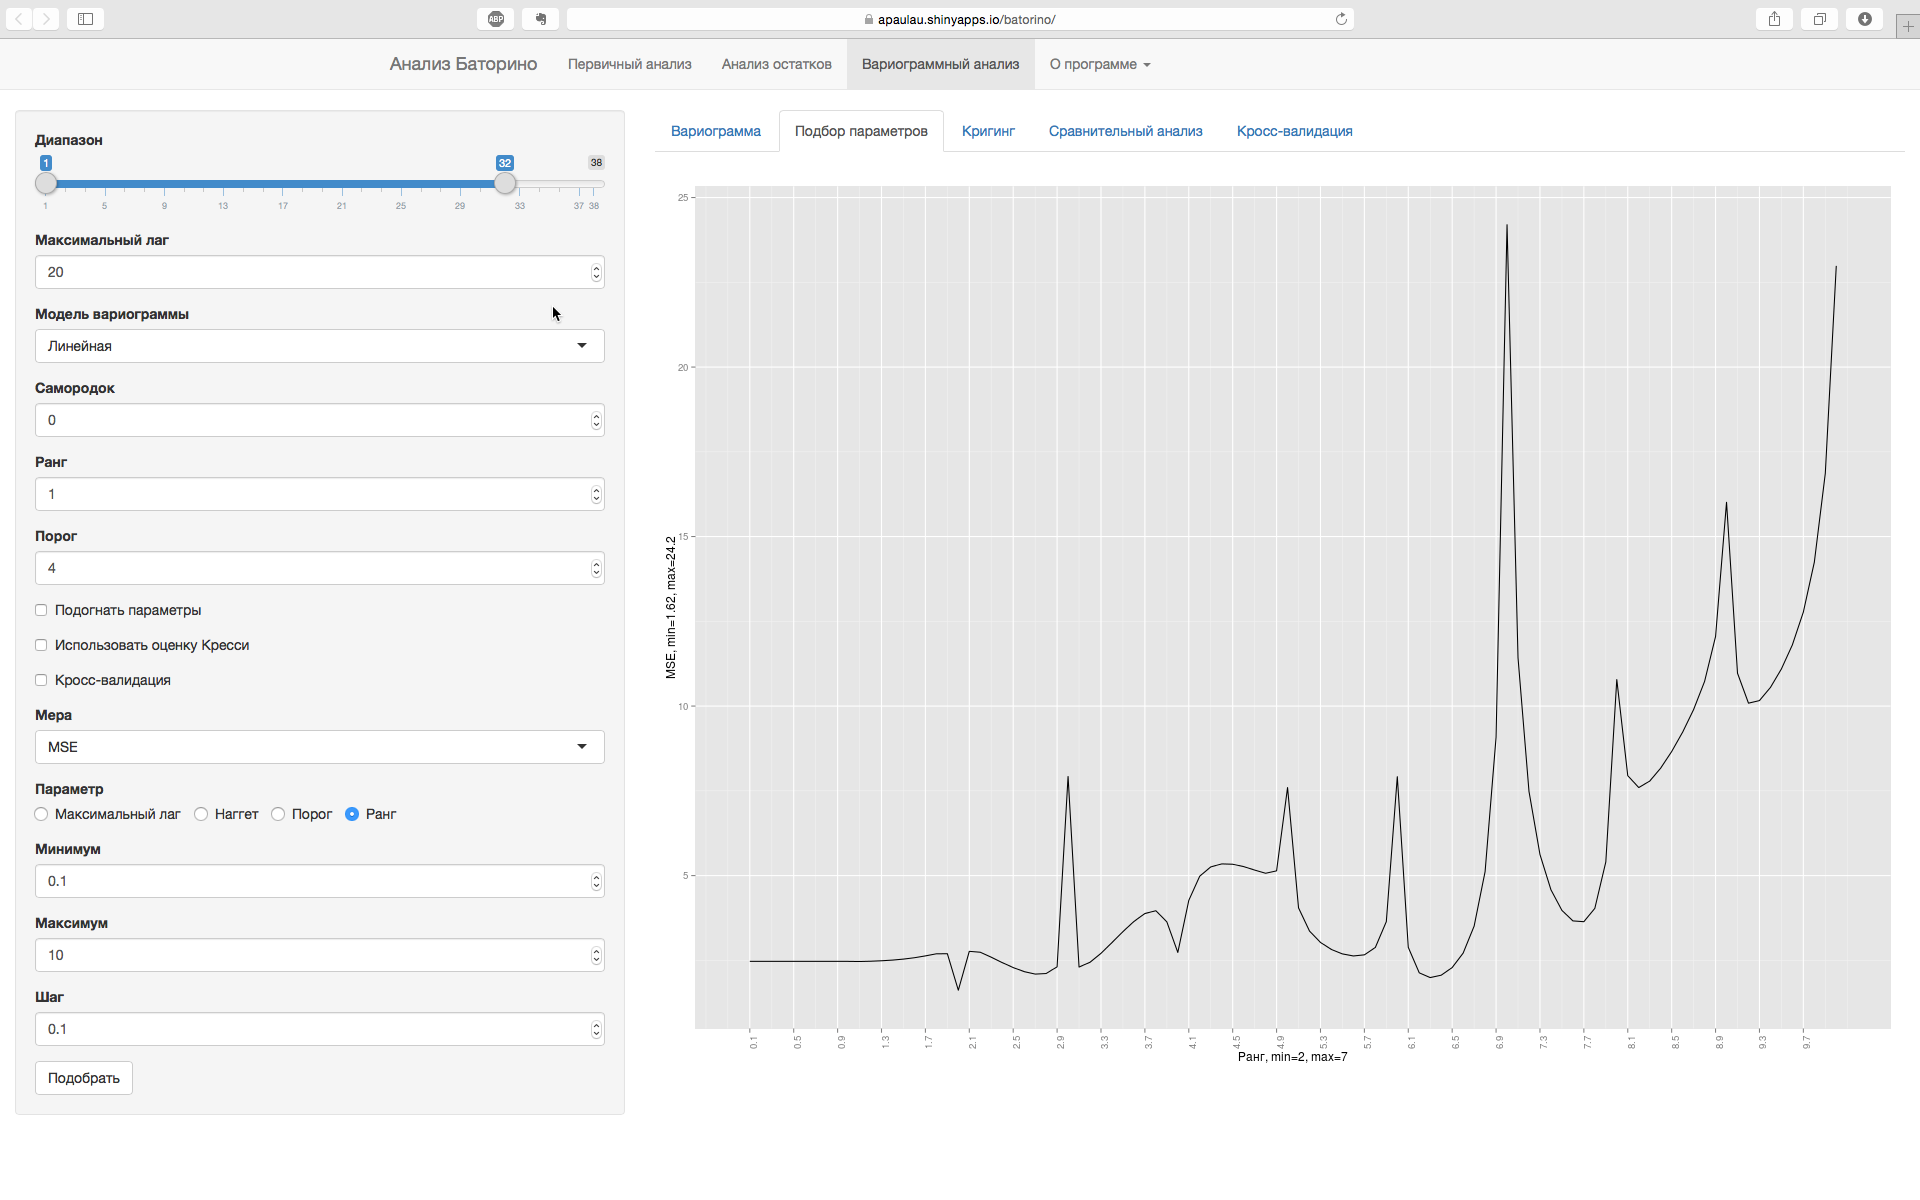
\includegraphics[width=1\linewidth]{../figures/static/5_fit.png}}
\caption{Подбор параметров модели вариограммы}
\label{img:mod_fit}
\end{figure}
С помощью таких статистик можно проследить, как изменяется качество модели при изменении какого-либо из параметров. Примерам вычисляемых статистик являются среднеквадратическое отклонение и коэффициент корреляции между фактическими и вычисленными значениями. Таким образом появляется возможность построения графика зависимости качества модели от исследуемого параметра. Это в свою очередь позволяет найти оптимальное значение искомого параметра и использовать его для подбора остальных. При втором подходе, адаптивном, в исследуемых данных отдаётся предпочтение последним наблюдениям. Для этого отбрасывается некоторое количество значений для последующего обучения модели. Подбор параметров осуществляется по статистикам, рассчитанным по отклонениям прогнозных значений от наблюдаемых. Таким образом достигается наилучший прогноз в краткосрочной перспективе. Побочным результатом, реализованного, является возможность оценить поведение модели при изменении одного из параметров.

Страница кригинга (рисунок \ref{img:mod_krige}) является наглядной демонстрацией применения всего вышеописанного. На ней изображается график с наблюдаемыми значениями и прогнозными значениями, вычисленными кригингом и по регрессионной модели.
\begin{figure}[ht]
\center{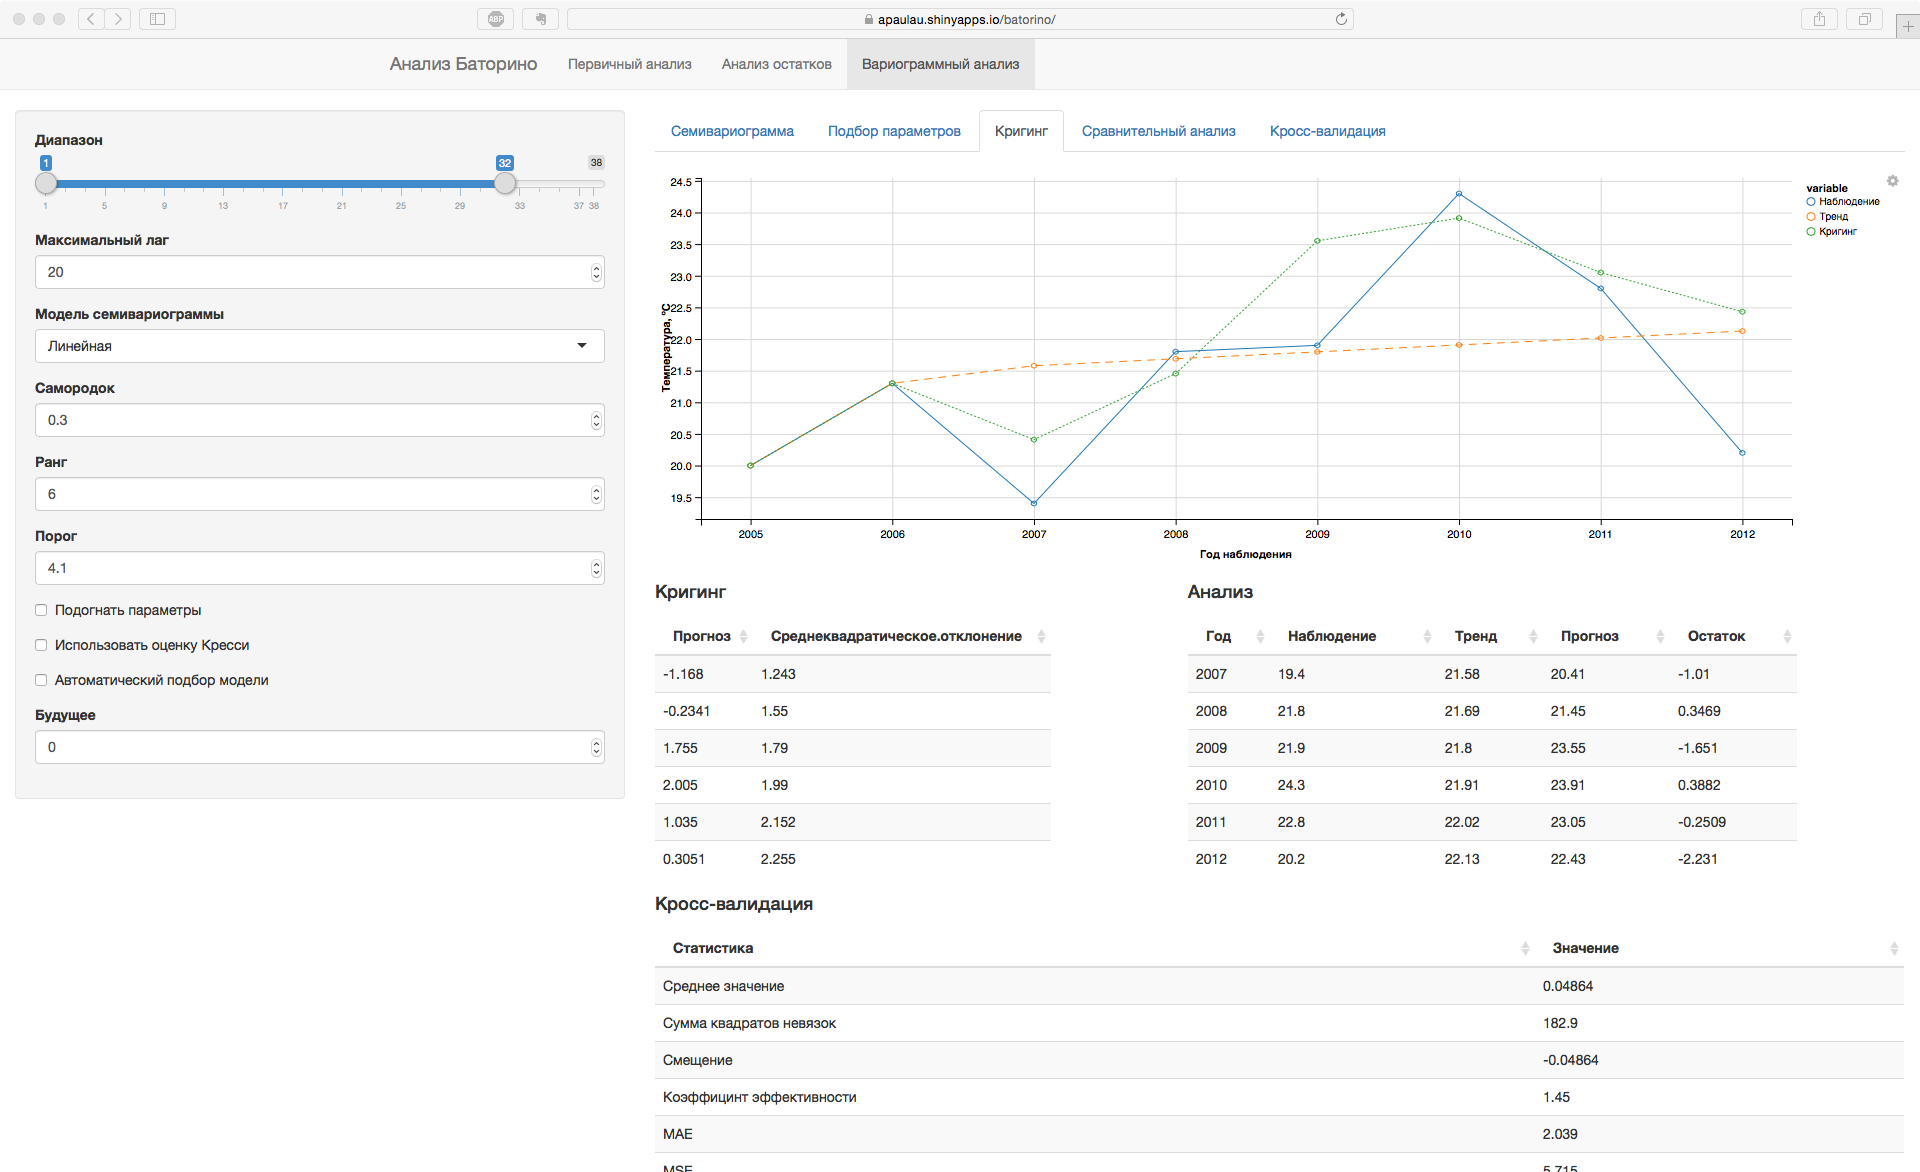
\includegraphics[width=1\linewidth]{../figures/static/6_krige.png}}
\caption{Подбор параметров модели вариограммы}
\label{img:mod_krige}
\end{figure}
Это позволяет оценить полученную модель и сделать различные заключения. График также сопровождается вспомогательными таблицами с произведёнными в процессе расчётами. В первую очередь это результаты кригинга с ошибкой для каждого из значений. Также отображается табличный вариант данных, изображённых на графики. И последняя таблица показывает значения статистик после применения кросс-валидации, что сразу позволяет сравнить конкретную модель с другими.

% section mod_variogram (end)